\documentclass[a4paper,11pt]{article}

\synctex=1 

\usepackage[margin=2.5cm]{geometry}
%[twoside,leqno,twocolumn]
\usepackage{amsthm}

%    Marcados dobles.
\usepackage{dsfont}     %\mathds{}, indicatriz. Double stroke font.
\usepackage{amssymb}     %\mathbb{}
\usepackage{bbm}        %\mathbbm{}, a variant font. See http://tug.ctan.org/macros/latex/contrib/bbm/bbm.pdf

%    Definiciones
\usepackage{mathtools}

%    Algoritmos
\usepackage{algorithm}
\usepackage{algorithmic}

% 	Long table
\usepackage{longtable}

%    Alineación de ecuaciones.
\usepackage{amsmath}

%    Listas
\usepackage{enumerate}

% CompactList
\usepackage{paralist}

%    Notación matemática
\usepackage{amsfonts}
\usepackage{amscd}

%    Colores
\usepackage{xcolor}

%    Subfigures
\usepackage{subcaption} % \begin{minipage}, \begin{subfigure}{.5\textwidth}

%   Drawings
\usepackage{tikz}
\usetikzlibrary{arrows,automata} % sub-packages

%   Define a shapes
\tikzstyle{rect} = [rectangle, rounded corners, minimum width=1cm, minimum height=1cm,text centered, draw=black ]
\tikzstyle{arrow} = [thick,->,>=stealth]

% Plots
\usepackage{pgfplots}
\pgfplotsset{compat=1.18}

%    URL's
\usepackage{hyperref}

% References
\usepackage{cleveref}

%    Abbreviations
\newcommand{\EE}{\mathbb{E}}
\newcommand{\ZZ}{\mathbb{Z}}
\newcommand{\PP}{\mathbb{P}}
\newcommand{\RR}{\mathbb{R}}
\newcommand{\NN}{\mathbb{N}}
\newcommand{\X}{\mathcal{X}}
\newcommand{\1}{\mathds{1}}
\newcommand{\m}{\mathbb}
\newcommand{\eps}{\varepsilon}
\newcommand{\defas}{\coloneqq}
\newcommand{\cond}{\;\middle\vert\;}
\newcommand{\until}{\, .. \,}
\DeclareMathOperator\supp{supp}

%    Document-abbreviations
\newcommand{\val}{\mathsf{val}} % val function
\newcommand{\LC}{\mathsf{LC}} % Leading coefficient
\newcommand{\wh}{\widehat}
\renewcommand{\vec}[1]{\boldsymbol{#1}} %    Vectors as bold leters

%    Strikeout text
\usepackage[normalem]{ulem} % \sout{} and \xout{}

%    Enumeration of theorems and styles
\theoremstyle{plain} % default: space up and down, italics inside.
\newtheorem{@theorem}{Theorem}[section]
\newenvironment{theorem}{\begin{@theorem}}{\end{@theorem}}
\newtheorem{Lemma}[@theorem]{Lemma}
\newtheorem{Corollary}[@theorem]{Corollary}
\newtheorem{Conjecture}[@theorem]{Conjecture}
\newtheorem{Proposition}[@theorem]{Proposition}

\theoremstyle{definition} % space up and down, roman inside.
\newtheorem{Definition}[@theorem]{Definition}
\newtheorem{Example}[@theorem]{Example}
\newtheorem{Condition}[@theorem]{Condition}
\newtheorem{Problem}[@theorem]{Problem}
\newtheorem{Exercise}[@theorem]{Exercise}

\theoremstyle{remark} % no space up and down, roman inside.
\newtheorem{Remark}[@theorem]{Remark}
\newtheorem{Note}[@theorem]{Note}
\newtheorem{Notation}[@theorem]{Notation}
\newtheorem{Claim}[@theorem]{Claim}
\newtheorem{Summary}[@theorem]{Summary}
\newtheorem{Cases}[@theorem]{Cases}
\newtheorem{Question}[@theorem]{Question}


%    Tables
\usepackage{multirow} %\multirow{number of rows}{width}{text}
\usepackage{hhline} %\hhline{| = | = | = |}

%    Pdf files included
\usepackage{pdfpages} % \includepdf[pages=-]{myfile.pdf}



\begin{document}

\title { 
    Population genomics of the critically endangered\\
    spoon-billed sandpiper\\
    Model calibration
    % \thanks{}  
}

\author { 
    Raimundo Saona\thanks{Institute of Science and Technology Austria}
    \and Anastasia Lyulina\thanks{Stanford University} 
    \and Fyodor Kondrashov*\thanks{Okinawa Institute of Science and Technology}
}

\date {
    \today
}


\maketitle

\begin{abstract}
	In this report we present the numerical approximation of the expectation of polymorphisms, also called heterozygosity, for a model of random selection coefficient.
	We present the model, and how to approximate all involved quantities step-by-step. 
\end{abstract}

\tableofcontents

\newpage


\section{Modeling}

We use the following notation.
\begin{itemize} 
	\item 
		selection coefficient $s$
	\item 
		dominance coefficient $h$
	\item 
		allele frequency $x$
	\item 
		mutation rate $U$
	\item 
		population size $N$
\end{itemize} 

Our parametric model for the distribution of the allele frequency is the following.
\[
	f(x \,|\, s, h) \propto \exp(2N s  ( x^2 + 2h x (1 - x) ) ) \, x^{4 N U - 1} \, (1 - x)^{4 N U - 1} \,.
\]
where we model $s$ by a mixture of a Gamma distribution with shape $\alpha$ and scale $1 / \beta$ (with negative sign), and a point mass at $s_0$ with probability $p$. 
In other words, 
\[
	S \sim \begin{cases}
		\delta_{s_0} 
			& p \\
		- \Gamma(\alpha, \beta)
			& 1 - p
	\end{cases}
\]
where $p$ is the probability of the mixture, and the Gamma distribution with shape $\alpha$ and scale $1 / \beta$ is given by
\[
	f_{\Gamma(\alpha, \beta)}(s) = x^{\alpha - 1} \exp(- \beta s) \frac{\beta^\alpha}{\Gamma(\alpha)} \1[s > 0]\,.
\]


The dominance coefficient $h$ is related to the selection coefficient as follows.
\[
	h = h(s) = \begin{cases}
		0
			& s = s_0 \\
		0.5
			& s \not = s_0
	\end{cases}
\]

We fix the following values.
\begin{itemize}
	\item $s_0 = - 1 \cdot 10^{-2}$ 
	\item $N = 2 \cdot 10^{4}$
	\item $U = 1.2 \cdot 10^{-8}$
\end{itemize}
so the model is parameterized by $p$, $\alpha$, and $\beta$.



\section{Polymorphisms}

Given a allele frequency $x$, a measure of polymorphisms is $2 x (1 - x)$. 
In our model, the allele frequency is a random variable $X$.
Therefore, the expected number of polymorphisms is 
\[
	\EE[poly] = \EE_{S} \left[ \EE_X \left[ 2 X (1 - X) \cond S \right] \right] \,.
\]
So $\EE[poly]$ can be approximated using a Monte Carlo approach by simulating the random selection coefficient $S$.








\section{Numerical approximation}

The following are key to derive formal error bounds on integrals.

\paragraph{Integration bounds.}
The following are simple but powerful results to numerically approximate integrals.

\begin{Proposition}
\label{Result: Square approximation}
	Consider $t > 0$ and a function $f \colon [0, t] \to \RR$.
	If $\| f - f(0)\|_\infty \le L$, then
	\[
		\left| \int_{[0, t]} f(x) dx - f(0) t \right| \le L t \,.
	\]
\end{Proposition}

\begin{Proposition}
	Consider $t > 0$ and functions $f, g \colon [0, t] \to \RR$.
	If $\| f - f(0)\|_\infty \le L$ and $\| g - g(0)\|_\infty \le L$, then
	\[
		\left| \int_{[0, t]} f(x) g(x) \, dx - f(0) g(0) t \right| \le L ( f(0) + g(0) ) t + L^2 t \,.
	\]
\end{Proposition}

%\begin{Proposition}
%	Consider a function $f \colon [0, 1] \to \RR$.
%	If $f$ is $L$-Lipschitz, then, for all $n \ge 1$, 
%	\[
%		\left| \int_{[0, 1]} f(x) \, dx - \sum_{i = 0}^{n-1} f(i/n) \frac{1}{n} \right| \le \frac{L}{2n} \,.
%	\]
%\end{Proposition}
%
%\begin{Proposition}
%	Consider a function $f \colon [0, 1] \to \RR$.
%	If $f$ is continuous, then
%	\[
%		\lim_{n \to \infty} \left| \int_{[0, 1]} f(x) dx - \sum_{i = 0}^{n-1} f(i/n) \frac{1}{n} \right| = 0 \,.
%	\]
%\end{Proposition}



\paragraph{Floating points.}
The IEEE Standard for Floating-Point Arithmetic (IEEE 754-2008) defines 64-bit floating point numbers, called ``binary64''.
These represent numbers in scientific notation in base $2$ with $1$ sing bit, $11$ exponent bits, and $53$ significand precision bits.
In other words, there are $15.95$ decimal digits of accuracy, for numbers whose exponent in base $10$ is in $[-308, 308]$.
The operations one can perform over floating point numbers losing only one binary digit of accuracy include addition, substraction, multiplication, division, exponentiation~\cite{goldberg1991WhatEveryComputer, tang1989TabledrivenImplementationExponential}, logarithmization~\cite{dedinechin2007FastCorrectlyRounded, lemaire2016ComputingFloatingpointLogarithms}, and arbitrary sum~\cite{zhu2010Algorithm908Online}.

For example, for all $n \ge 1$ and $x_1, x_2, \ldots, x_n \in \RR$ such that $10^{-308} \le |x_i| \le 308$, we can compute
\[
	\sum_{i = 0}^{n} \exp(x_i)
\]
losing only at most two binary digits of accuracy.



\paragraph{Normalizing constant.}
Consider 
\[
	C(s, h) 
		= \int_{[0, 1]} g(x \mid s, h) \,dx 
		= \int_{[0, 1]} \exp(2N s ( x^2 + 2h x (1 - x) ) ) \, x^{4 N U - 1} \, (1 - x)^{4 N U - 1} \, dx \,,
\]
the normalizing constant of $f(x \mid s, h)$.

Note that $g( \, \cdot \mid s, h)$ is a function with singularities at $0$ and $1$.
To numerically deal with this, $C(s, h)$ can be written as a numerically stable expression as follows.
\begin{align*}
	C(s, h) 
		&= \int_{[0, 1]} g(x \mid s, h) \,dx \\
		&= \int_{[0, 1/2]} g(x \mid s, h) \,dx + \int_{[1/2, 1]} g(x \mid s, h) \,dx \\
		&= \int_{[0, 1/2]} g(x \mid s, h) - x^{4 N U - 1} \,dx + \int_{[0, 1/2]} x^{4 N U - 1} \, dx \\
		&\qquad + \int_{[1/2, 1]} g(x \mid s, h) - \exp( 2 N s )(1 - x)^{4 N U - 1} \,dx + \exp( 2 N s ) \int_{[1/2, 1]} (1 - x)^{4 N U - 1} \,dx \\
		&= \int_{[0, 1/2]} g(x \mid s, h) - x^{4 N U - 1} \,dx + \int_{[1/2, 1]} g(x \mid s, h) - \exp( 2 N s )(1 - x)^{4 N U - 1} \,dx \\
		&\qquad + \left( 1 + \exp( 2 N s ) \right) \int_{[0, 1/2]} x^{4 N U - 1} \, dx \\
		&= \int_{[0, 1/2]} g(x \mid s, h) - x^{4 N U - 1} \,dx + \int_{[1/2, 1]} g(x \mid s, h) - \exp( 2 N s )(1 - x)^{4 N U - 1} \,dx \\
		&\qquad + \big( 1 + \exp( 2 N s ) \big) \frac{1}{4 N U} \left(\frac{1}{2}\right)^{4 N U} \,.
\end{align*}
This expression is stable because all integrands are continuous and have no singularities.
See \Cref{Figure: Normalizing constant} for an illustration.

\begin{figure}[h]
\centering
	\pgfplotsset{width=5cm}
	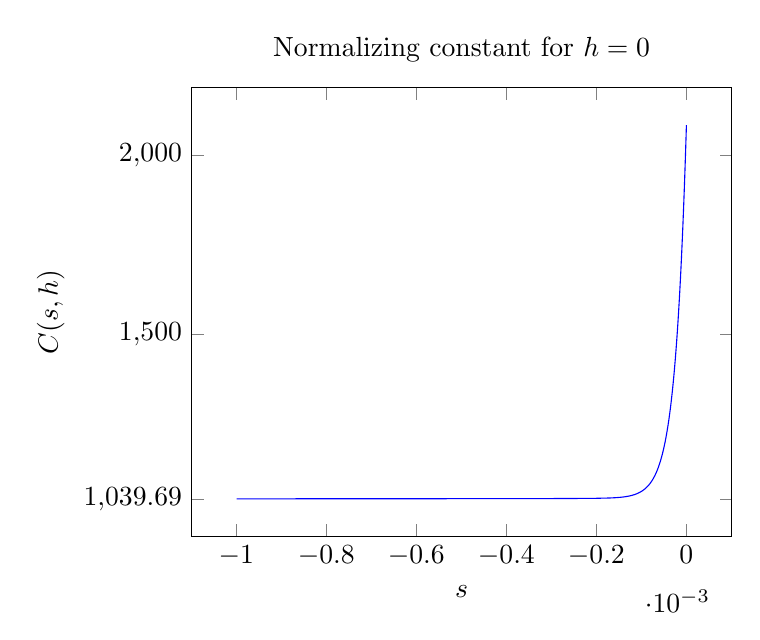
\begin{tikzpicture}
		\begin{axis}[
			title = {Normalizing constant for $h = 0$},
			xlabel = {$s$},
			ylabel = {$C(s, h)$},
			ytick = {1039.69, 1500, 2000},
		]
			\addplot [blue] coordinates {
				(-0, 2083.330179486882)
				(-0.000001, 2042.5243906108783)
				(-0.000002, 2003.3173429858145)
				(-0.000003, 1965.6463761016203)
				(-0.000004, 1929.4512856729446)
				(-0.000005, 1894.6742273510117)
				(-0.000006, 1861.2596242102986)
				(-0.000007, 1829.1540778620404)
				(-0.000008, 1798.3062830523838)
				(-0.000009, 1768.666945608564)
				(-0.00001, 1740.188703601857)
				(-0.000011, 1712.8260516011903)
				(-0.000012, 1686.5352678962458)
				(-0.000013, 1661.2743445736407)
				(-0.000014, 1637.002920334327)
				(-0.000015, 1613.6822159447527)
				(-0.000016, 1591.2749722185154)
				(-0.000017, 1569.7453904293202)
				(-0.000018, 1549.059075059908)
				(-0.000019, 1529.1829787953845)
				(-0.00002, 1510.08534967296)
				(-0.000021, 1491.7356803035525)
				(-0.000022, 1474.10465908404)
				(-0.000023, 1457.1641233221094)
				(-0.000024, 1440.887014198731)
				(-0.000025, 1425.2473334962062)
				(-0.000026, 1410.2201020225812)
				(-0.000027, 1395.7813196659163)
				(-0.000028, 1381.9079270145157)
				(-0.000029, 1368.577768481728)
				(-0.00003, 1355.7695568763309)
				(-0.000031, 1343.4628393618282)
				(-0.000032, 1331.6379647502104)
				(-0.000033, 1320.2760520778606)
				(-0.000034, 1309.3589604133454)
				(-0.000035, 1298.8692598487896)
				(-0.000036, 1288.790203628441)
				(-0.000037, 1279.1057013698426)
				(-0.000038, 1269.8002933347723)
				(-0.000039, 1260.859125708807)
				(-0.00004, 1252.2679268499546)
				(-0.000041, 1244.0129844683806)
				(-0.000042, 1236.081123700713)
				(-0.000043, 1228.459686043864)
				(-0.000044, 1221.1365091146665)
				(-0.000045, 1214.0999072029617)
				(-0.000046, 1207.338652587016)
				(-0.000047, 1200.841957581397)
				(-0.000048, 1194.5994572885857)
				(-0.000049, 1188.6011930267384)
				(-0.00005, 1182.8375964070935)
				(-0.000051, 1177.29947403555)
				(-0.000052, 1171.9779928139571)
				(-0.000053, 1166.8646658175937)
				(-0.000054, 1161.9513387262625)
				(-0.000055, 1157.230176787282)
				(-0.000056, 1152.6936522895387)
				(-0.000057, 1148.3345325285507)
				(-0.000058, 1144.1458682433063)
				(-0.000059, 1140.1209825063754)
				(-0.00006, 1136.253460049527)
				(-0.000061, 1132.5371370077783)
				(-0.000062, 1128.9660910654775)
				(-0.000063, 1125.5346319886503)
				(-0.000064, 1122.237292528479)
				(-0.000065, 1119.0688196813533)
				(-0.000066, 1116.024166291526)
				(-0.000067, 1113.0984829829365)
				(-0.000068, 1110.2871104072951)
				(-0.000069, 1107.58557179604)
				(-0.00007, 1104.9895658042456)
				(-0.000071, 1102.4949596350423)
				(-0.000072, 1100.0977824335482)
				(-0.000073, 1097.79421893975)
				(-0.000074, 1095.5806033901827)
				(-0.000075, 1093.453413658648)
				(-0.000076, 1091.4092656266128)
				(-0.000077, 1089.4449077742715)
				(-0.000078, 1087.5572159836331)
				(-0.000079, 1085.7431885453082)
				(-0.00008, 1083.999941361029)
				(-0.000081, 1082.3247033342104)
				(-0.000082, 1080.7148119411938)
				(-0.000083, 1079.1677089760858)
				(-0.000084, 1077.6809364623862)
				(-0.000085, 1076.252132724871)
				(-0.000086, 1074.8790286154424)
				(-0.000087, 1073.5594438869168)
				(-0.000088, 1072.2912837089457)
				(-0.000089, 1071.072535320502)
				(-0.00009, 1069.9012648135777)
				(-0.000091, 1068.7756140429462)
				(-0.000092, 1067.6937976570532)
				(-0.000093, 1066.6541002452816)
				(-0.000094, 1065.6548735970343)
				(-0.000095, 1064.6945340682487)
				(-0.000096, 1063.7715600511308)
				(-0.000097, 1062.8844895430664)
				(-0.000098, 1062.0319178108164)
				(-0.000099, 1061.2124951462672)
				(-0.0001, 1060.4249247101434)
				(-0.000101, 1059.6679604602336)
				(-0.000102, 1058.9404051608221)
				(-0.000103, 1058.2411084701369)
				(-0.000104, 1057.56896510276)
				(-0.000106, 1056.3019319538278)
				(-0.000108, 1055.1312991746047)
				(-0.00011, 1054.0496750934008)
				(-0.000112, 1053.0502356641034)
				(-0.000114, 1052.1266808545809)
				(-0.000116, 1051.2731943865974)
				(-0.000119, 1050.1127102423998)
				(-0.000122, 1049.0814778419397)
				(-0.000125, 1048.1649341564334)
				(-0.000129, 1047.0991652937644)
				(-0.000133, 1046.1878237038593)
				(-0.000139, 1045.0615740002215)
				(-0.000146, 1044.0397436098785)
				(-0.000155, 1043.0723757173546)
				(-0.00017, 1042.0410345274015)
				(-0.000206, 1041.0015859352602)
				(-0.000283, 1040.5038491694768)
				(-0.000323, 1040.4015049705272)
				(-0.000374, 1040.3000910285468)
				(-0.000435, 1040.2004593121303)
				(-0.000508, 1040.1010504110689)
				(-0.000597, 1040.000036562812)
				(-0.000647, 1039.950520864286)
				(-0.000702, 1039.9007928080903)
				(-0.000763, 1039.850491351597)
				(-0.00083, 1039.8001464051436)
				(-0.000918, 1039.7404427312226)
				(-0.000934, 1039.7302649865521)
				(-0.00095, 1039.720276511378)
				(-0.000966, 1039.7104705078823)
				(-0.000983, 1039.7002443657248)
				(-0.000999, 1039.6907947406796)
			};
		\end{axis}
	\end{tikzpicture}
	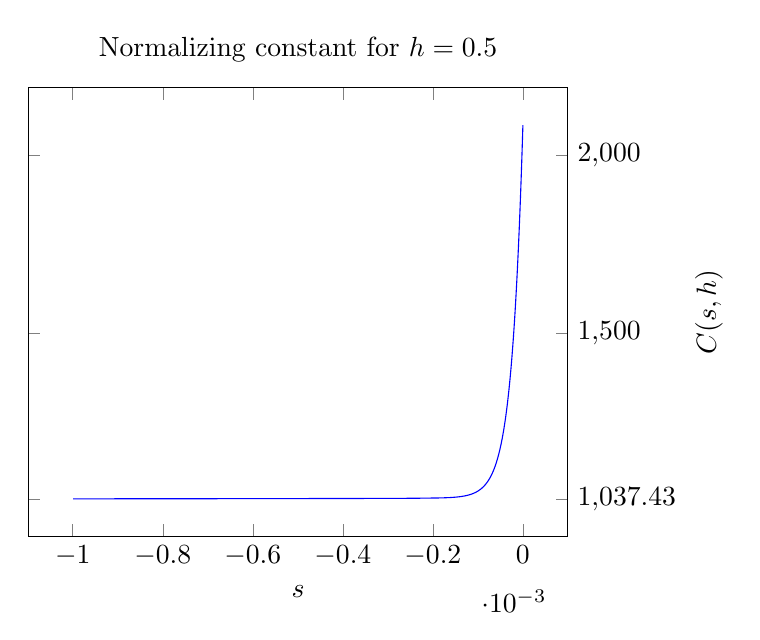
\begin{tikzpicture}
		\begin{axis}[
			title = {Normalizing constant for $h = 0.5$},
			xlabel = {$s$},
			ylabel = {$C(s, h)$},
			ytick = {1037.43, 1500, 2000},
			yticklabel pos=upper,
		]
			\addplot [blue] coordinates {
				(-0, 2083.330179486882)
				(-0.000001, 2042.4851244127628)
				(-0.000002, 2003.2400923706514)
				(-0.000003, 1965.532375644298)
				(-0.000004, 1929.3017245358858)
				(-0.000005, 1894.4902510088684)
				(-0.000006, 1861.042336108303)
				(-0.000007, 1828.904541010579)
				(-0.000008, 1798.0255215602617)
				(-0.000009, 1768.3559461573357)
				(-0.00001, 1739.8484168635025)
				(-0.000011, 1712.457393601327)
				(-0.000012, 1686.139121324986)
				(-0.000013, 1660.8515600461176)
				(-0.000014, 1636.5543176028375)
				(-0.000015, 1613.2085850643853)
				(-0.000016, 1590.777074668064)
				(-0.000017, 1569.2239601892106)
				(-0.000018, 1548.5148196487999)
				(-0.000019, 1528.6165802670423)
				(-0.00002, 1509.4974655749327)
				(-0.000021, 1491.1269445991334)
				(-0.000022, 1473.4756830389265)
				(-0.000023, 1456.5154963571251)
				(-0.000024, 1440.2193047099204)
				(-0.000025, 1424.5610896435621)
				(-0.000026, 1409.5158524886135)
				(-0.000027, 1395.0595743852286)
				(-0.000028, 1381.1691778755053)
				(-0.000029, 1367.822490001485)
				(-0.00003, 1354.9982068497718)
				(-0.000031, 1342.675859486055)
				(-0.000032, 1330.8357812250515)
				(-0.000033, 1319.4590761835102)
				(-0.000034, 1308.5275890659843)
				(-0.000035, 1298.0238761350363)
				(-0.000036, 1287.9311773194468)
				(-0.000037, 1278.2333894158148)
				(-0.000038, 1268.9150403406816)
				(-0.000039, 1259.9612643919966)
				(-0.00004, 1251.357778480356)
				(-0.000041, 1243.0908592919973)
				(-0.000042, 1235.1473213470201)
				(-0.000043, 1227.5144959177408)
				(-0.000044, 1220.1802107734568)
				(-0.000045, 1213.1327707192313)
				(-0.000046, 1206.360938897561)
				(-0.000047, 1199.853918823027)
				(-0.000048, 1193.6013371211902)
				(-0.000049, 1187.5932269441282)
				(-0.00005, 1181.82001203608)
				(-0.000051, 1176.2724914237199)
				(-0.000052, 1170.941824706571)
				(-0.000053, 1165.8195179240297)
				(-0.000054, 1160.8974099764014)
				(-0.000055, 1156.1676595782233)
				(-0.000056, 1151.6227327230154)
				(-0.000057, 1147.2553906393991)
				(-0.000058, 1143.0586782193354)
				(-0.000059, 1139.0259128999617)
				(-0.00006, 1135.1506739812537)
				(-0.000061, 1131.4267923624236)
				(-0.000062, 1127.8483406806404)
				(-0.000063, 1124.409623836301)
				(-0.000064, 1121.1051698896993)
				(-0.000065, 1117.9297213145303)
				(-0.000066, 1114.8782265942473)
				(-0.000067, 1111.9458321478269)
				(-0.000068, 1109.1278745720285)
				(-0.000069, 1106.419873187745)
				(-0.00007, 1103.8175228785208)
				(-0.000071, 1101.3166872097866)
				(-0.000072, 1098.9133918178027)
				(-0.000073, 1096.603818057742)
				(-0.000074, 1094.3842969007533)
				(-0.000075, 1092.2513030702412)
				(-0.000076, 1090.2014494079917)
				(-0.000077, 1088.2314814611275)
				(-0.000078, 1086.3382722812398)
				(-0.000079, 1084.518817427376)
				(-0.00008, 1082.7702301648976)
				(-0.000081, 1081.0897368525243)
				(-0.000082, 1079.4746725101904)
				(-0.000083, 1077.9224765606261)
				(-0.000084, 1076.430688737851)
				(-0.000085, 1074.9969451560403)
				(-0.000086, 1073.6189745324748)
				(-0.000087, 1072.2945945585354)
				(-0.000088, 1071.0217084129388)
				(-0.000089, 1069.7983014116376)
				(-0.000093, 1065.3618692126001)
				(-0.000098, 1060.7185006242892)
				(-0.000101, 1058.3424594412281)
				(-0.000104, 1056.2318081922324)
				(-0.000107, 1054.356625220316)
				(-0.000111, 1052.1772279690695)
				(-0.000115, 1050.314816345783)
				(-0.000118, 1049.0976704637922)
				(-0.000121, 1048.0153166864725)
				(-0.000124, 1047.052580466167)
				(-0.000127, 1046.196000222444)
				(-0.000131, 1045.198581161245)
				(-0.000136, 1044.1503606381366)
				(-0.000142, 1043.1315574591229)
				(-0.00015, 1042.089455137766)
				(-0.000162, 1041.010358046453)
				(-0.000181, 1040.0257947783202)
				(-0.000242, 1039.0061026280468)
				(-0.000361, 1038.500459941787)
				(-0.000578, 1038.0012737427649)
				(-0.000607, 1037.950234573971)
				(-0.000637, 1037.9000582091533)
				(-0.000701, 1037.8008012989005)
				(-0.000772, 1037.7011742481793)
				(-0.000851, 1037.600926066207)
				(-0.000939, 1037.5000039221293)
				(-0.000948, 1037.4902370750835)
				(-0.000957, 1037.480565242051)
				(-0.000966, 1037.470986591486)
				(-0.000976, 1037.4604507723889)
				(-0.000986, 1037.4500254308048)
				(-0.000995, 1037.4407351844782)
				(-0.000999, 1037.4366338875002)
			};
		\end{axis}
	\end{tikzpicture}
	\caption{Normalizing constant in terms of $s$}
	\label{Figure: Normalizing constant}
\end{figure}

\paragraph{Fixed s and h.}

Fix $s, h$ such that $|2Ns| < 1000$, i.e., $|s| < 1/40 = 25 \cdot 10^{-2}$. 
We are interested in in computing
\begin{align*}
	\EE \left[ poly \cond s, h \right] 
		&= \EE_X \left[ 2 X (1 - X) \cond s, h \right] \\
		&= \int_{[0, 1]} 2 x (1 - x) \frac{ f(x \mid s, h) }{ C(s, h) } dx \\
		&= \int_{[0, 1]}  2 x (1 - x) \frac{ \exp( 2 N s ( x^2 + 2h x(1-x) ) ) \, x^{4 N U - 1} \, (1 - x)^{4 N U - 1} }{ C(s, h) } \, dx \\
		&= \frac{2}{C(s, h)} \int_{[0, 1]}  \exp( 2 N s ( x^2 + 2h x(1-x)) ) \, x^{4 N U} \, (1 - x)^{4 N U} \, dx \\
		&= \frac{2}{C(s, h)} \int_{[0, 1]}  \exp( 4 N U \ln(x (1-x)) + 2 N s ( x^2 + 2h x(1-x)) ) \, dx \,,
\end{align*}

We show how to approximate
\[
	\int_{[0, 1]}  \exp( 4 N U \ln(x (1-x)) +  ) \, dx \,.
\]

First, we notice that we are interested in $s \in [-0.01, 0]$ and $h \in [0, 1/2]$.
Second, the integration in $[0, 1/2]$ is harder to approximate than the integration in $[1/2, 1]$ since the exponential $\exp(2 N s ( x^2 + 2h x(1-x)))$ is smaller for $x$ large.
Therefore, we present in detail how to approximate the integration over $[0, 1/2]$.
Note that, for $s \le 0$, $h \in [0, 1/2]$, and $x \in [0, 1]$, we have that
\begin{align*}
	\exp( 2 N s ( x^2 + 2h x(1-x))  )
		&\le 1 \\
	 x^{4 N U} 
	 	&\le 1 \\
 	(1 - x)^{4 N U} 
 		&\le 1 \,.
\end{align*}
Therefore,
\[
		\EE \left[ poly \cond s, h \right] 
			\le \frac{2}{C(s, h)} \,.
\]

The integral over $[0, 1/2]$ can be approximated as usual by a sum over a grid $0 = x_0 < x_1 < \ldots < x_n = 1/2$.
Note that, for every $0 < x_1 < x_2 < 1/2$, 
\[
	\sup_{x \in [x_1, x_2]}\left| \frac{\partial}{\partial x} \exp( 2 N s ( x^2 + 2h x(1-x)) ) \, x^{4 N U} \, (1 - x)^{4 N U} \right| 
		\le 4N \left( \frac{U}{x_1} + s \right) \,.
\]
Therefore, by \Cref{Result: Square approximation}, 
\begin{align*}
	&\int_{[x_1, x_2]}  \exp( 2 N s ( x^2 + 2h x(1-x)) ) \, x^{4 N U} \, (1 - x)^{4 N U} \, dx  \\
		&\qquad \approx (x_2 - x_1) \exp( 2 N s ( x_1^2 + 2 h x_1 (1 - x_1)) ) \, x_1^{4 N U} \, (1 - x_1)^{4 N U} \,,
\end{align*}
where the approximation error is no larger than $(x_2 - x_1)^2 4 N (U / x_1 + |s|)$. 
We control this error by choosing an appropiate grid.
For the initial and last intervals in our grid, by a simple bound for $s < 0$,
\[
	\left | \int_{[0, x_1]} \exp( 2 N s ( x^2 + 2h x(1-x)) ) \, x^{4 N U} \, (1 - x)^{4 N U} \, dx \right | 
		< x_1 \,.
\]
Therefore, the overall error by using a grid and the simplest approximation of the integral is
\[
	x_1 
		+ \sum_{i = 1}^{n - 1} (x_{i + 1} - x_i)^2 4 N  \left( \frac{U}{x_i} + |s| \right) \,.
\]

For $\eps \in (0, 1)$, define $x_1 \defas \eps$ and 
\[
	x_{i + 1} \defas \sqrt{\eps} \sqrt{x_i} + x_i \,.
\]
This grid satisfies that $(x_{i + 1} - x_i)^2 / x_i = \eps$. 
Therefore, this grid incurs in at most the following approximation error of the integral
\[
	\eps 
		+ \sum_{i = 1}^{n(\eps)-1} \eps 4N (U + |s|) 
	< \eps \left(1 + n(\eps) 4 N (U + |s|) \right) \,,
\]
where $n(\eps)$ is number of points required so that $x_{n(\eps)} \ge 1/2$, which converges to zero as $\eps$ converges to zero. 

Note that, the smaller $\eps$, the smaller the numbers $x_1$ we need to consider.
As we work with 64-bits floating points, there is a limit to how small we can consider $\eps$.
We keep track of the error estimation to ensure that the overall error is less than $10^{-6}$.
See \Cref{Figure: Integration approximation error fast} for a plot of the behaviour of the approximation error of the integral in terms of $\eps$.

\begin{figure}[h]
	\centering
	\pgfplotsset{width=7cm}
	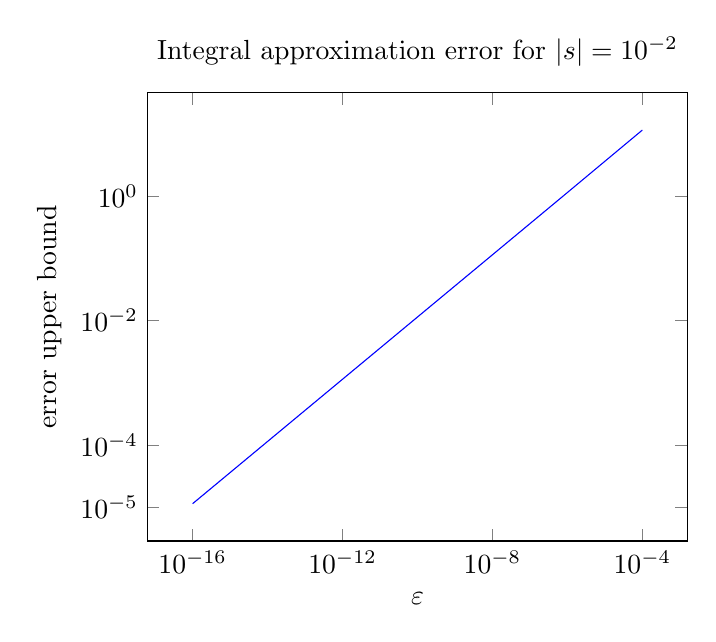
\begin{tikzpicture}
		\begin{loglogaxis}[
			title = {Integral approximation error for $|s| = 10^{-2}$},
			xlabel = {$\eps$},
			xtick = {0.0001, 0.00000001, 0.000000000001, 0.0000000000000001},
			ylabel = {error upper bound},
			ytick = {100, 1, 0.01, 0.0001, 0.00001},
			]
			\addplot [blue] coordinates {
				(0.0001,11.4401)
				(0.000001,1.1336)
				(0.00000001,0.11316)
				(0.00000000000001,0.00011313)
				(0.0000000000000001,0.000011313)
			};
			% Code
			% ```python
			%	eps = 1e-16
			%	n = 1
			%	x = eps
			%	factor = eps
			%	while x < 1/2:
			%	n = n + 1
			%	x = math.sqrt( factor * x) + x
			%	
			%	
			%	N = 2e4
			%	U = 1.2e-8
			%	s = 1e-2
			%	
			%	eps * (1 + n * 4 * N * (U + s))
			% ```
		\end{loglogaxis}
	\end{tikzpicture}
	\caption{Plot of the normalizing constant}
	\label{Figure: Integration approximation error fast}
\end{figure}

Note that, if $\eps \ge 10^{-16}$, then $n(\eps) < 2 \cdot 10^8$, so the required number of evaluations is manageable in modern computers.
Recall that, each evaluation must be within the range of 64-bit floating point numbers.
This is the case because, for $s \in [-1 \cdot 10^{-2}, 0]$ and $h \in [0, 0.5]$, we have that, for all $x \in [10^{-16}, 1/2]$,
\[
	|4 N U \ln(x (1-x)) + 2 N s ( x^2 + 2h x(1-x))| \le |4 N U \ln(x)| + |2 N s ( x^2 + x )| \le 301 \,,
\]
so the integrand involving the exponential is within the 64-bit floating point range. 

In summary, taking $\eps = 10^{-16}$, we have shown that, for $s \in [-1 \cdot 10^{-2}, 0]$ and $h \in [0, 1/2]$,
\begin{align*}
	&\int_{[0, 1/2]}  \exp( 4 N U \ln(x (1-x)) + 2 N s ( x^2 + 2h x(1-x)) ) \, dx \\
	&\quad
	\approx \sum_{i = 1}^{n(10^{-15}) - 1} (x_{i+1} - x_i) \exp( 4 N U \ln(x_i (1-x_i)) + 2 N s ( x_i^2 + 2h x_i (1 - x_i)) ) \,,
\end{align*}
and the approximation error is less than $10^{-5}$.

To obtain this sum with an appropiate accuracy, note that $x_i$ is represented in 64-bit floating point, which has at least $15.9$ digits of accuracy. 
Then, while computing this expression naively, we lose at most $12$ binary digits, which corresponds to at most $4$ digits of accuracy.
In other words, we can obtain this approximation with $11$ digits of accuracy. 

The integral over $[1/2, 1]$ can be approximated using similar bounds.
Finally, together with an appropiate approximation of $C(s, h)$, we can compute $\EE \left[ poly \cond s, h \right]$ with an error of at most $10^{-5}$.
\Cref{Figure: Epected poly given s for h = 0.0} and \Cref{Figure: Epected poly given s for h = 0.5} visualize the approximation for $h = 0.0$ and $h = 0.5$ respectively.

\begin{figure}[h]
	\centering
	\pgfplotsset{width=5cm}
	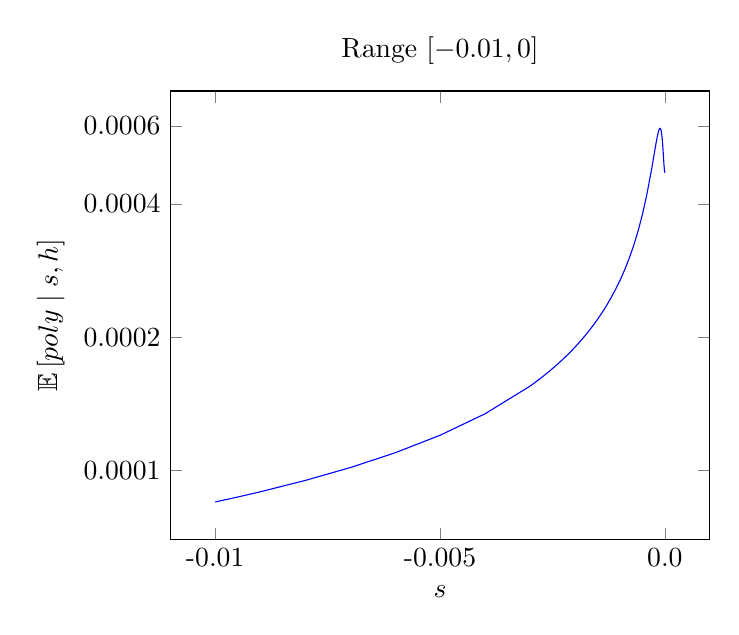
\begin{tikzpicture}
		\begin{semilogyaxis}[
				title = {Range $[-0.01, 0]$},
				ylabel = {$\EE \left[ poly \cond s, h \right]$},
				ytick = {0.0006, 0.0004, 0.0002, 0.0001},
				yticklabels = {0.0006, 0.0004, 0.0002, 0.0001},
				xlabel = {$s$},
				xtick = {-0.01, -0.005, 0.0},
				xticklabels = {-0.01, -0.005, 0.0}, scaled x ticks=false,
			]
			\addplot [blue] table {
                                -0.01                   0.00008501514709555435
                                -0.0099                 0.00008544340608278284
                                -0.0098                 0.00008587820311172771
                                -0.0097                 0.00008631970625093858
                                -0.0096                 0.00008676808968044427
                                -0.0095                 0.00008722353398048142
                                -0.0094                 0.00008768622643707226
                                -0.0093                 0.00008815636136562528
                                -0.0092                 0.00008863414045382948
                                -0.0091                 0.00008911977312521615
                                -0.009                  0.00008961347692487662
                                -0.008                  0.00009504899730087913
                                -0.007                  0.00010161107104511563
                                -0.006                  0.00010975171794770189
                                -0.005                  0.0001202258732131884
                                -0.004                  0.00013441491702193768
                                -0.003                  0.00015520607305443242
                                -0.003                  0.00015520607305443242
                                -0.0029                 0.00015785898051424397
                                -0.0028                 0.00016065275363878515
                                -0.0027                 0.00016360031716145307
                                -0.0026                 0.00016671631941294316
                                -0.0025                 0.00017001743957475836
                                -0.0024                 0.00017352276464267127
                                -0.0023                 0.00017725425559726084
                                -0.0022                 0.000181237328853968
                                -0.0021                 0.00018550158827175019
                                -0.002                  0.0001900817560718053
                                -0.0019                 0.00019501886986256862
                                -0.0018                 0.00020036184058378544
                                -0.0017                 0.0002061695073834939
                                -0.0016                 0.00021251338811052555
                                -0.0015                 0.00021948142143628598
                                -0.0014                 0.00022718315118400246
                                -0.0013                 0.00023575705467302483
                                -0.0012                 0.0002453811349680308
                                -0.0011                 0.0002562886084930104
                                -0.001                  0.00026879175372652444
                                -0.0009                 0.00028331915090015124
                                -0.0008                 0.00030047531130410844
                                -0.0007                 0.0003211379400940495
                                -0.0006                 0.0003466166674521268
                                -0.0005                 0.0003788995834447302
                                -0.0004                 0.0004209537013639709
                                -0.0003                 0.0004765846696792525
                                -0.00029                        0.00048301019846077464
                                -0.00028                        0.0004895903402668485
                                -0.00027                        0.0004963191734383967
                                -0.00026                        0.0005031878886341686
                                -0.00025                        0.0005101840857221512
                                -0.00024                        0.0005172909078969085
                                -0.00023                        0.000524485974114417
                                -0.00022                        0.0005317400623505819
                                -0.00021                        0.0005390154847165423
                                -0.0002                 0.0005462640827368618
                                -0.00019                        0.0005534247574748073
                                -0.00018                        0.0005604204355014928
                                -0.00017                        0.0005671543610822852
                                -0.00016                        0.0005735056087063938
                                -0.00015                        0.0005793237405968988
                                -0.00014                        0.0005844226196004826
                                -0.00013                        0.0005885735941160031
                                -0.00012                        0.0005914986936467291
                                -0.00011                        0.0005928652916217373
                                -0.0001                 0.0005922851736485207
                                -0.00009                        0.0005893235283430916
                                -0.00008                        0.0005835273589598799
                                -0.00007                        0.0005744881951830009
                                -0.00006                        0.000561958801487218
                                -0.00005                        0.0005460416965322386
                                -0.00004                        0.0005274456035118235
                                -0.00003                        0.0005077477505613694
                                -0.00002                        0.0004895112022593879
                                -0.00001                        0.0004760904786845811
                                -0.000009                       0.0004751586534256445
                                -0.000008                       0.0004743189575508033
                                -0.000007                       0.0004735772121025261
                                -0.000006                       0.00047294057062432295
                                -0.000005                       0.00047241857525599193
                                -0.000004                       0.0004720254077002949
                                -0.000003                       0.00047178542815747184
                                -0.000002                       0.0004717502507929271
                                -0.000001                       0.00047207893557613253
                                -0.0000009                      0.0004721505057865423
                                -0.0000008                      0.000472234506840612
                                -0.0000007                      0.0004723339880430206
                                -0.0000006                      0.00047245341081619363
                                -0.0000005                      0.00047259968576005614
                                -0.0000004                      0.00047278438010174735
                                -0.0000003                      0.00047302915859703343
                                -0.0000002                      0.000473382606117568
                                -0.0000001                      0.00047399940914860975
                                -0.00000009                     0.0004740939257882394
                                -0.00000008                     0.00047419971410839277
                                -0.00000007                     0.000474319756924066
                                -0.00000006                     0.0004744584050349582
                                -0.00000005                     0.0004746223431523665
                                -0.00000004                     0.0004748226248735699
                                -0.00000003                     0.0004750325097726186
                                -0.00000002                     0.0004750320834016828
                                -0.00000001                     0.00047503166662056224
                                -0.000000009                    0.00047503162546992835
                                -0.000000008                    0.0004750315844152037
                                -0.000000007                    0.00047503154345638905
                                -0.000000006                    0.0004750315025934855
                                -0.000000005                    0.00047503146182649404
                                -0.000000004                    0.00047503142115541577
                                -0.000000003                    0.0004750313805802515
                                -0.000000002                    0.0004750313401010024
                                -0.000000001                    0.0004750312997176693
                                0                       0.0004750312594302533
			};
		\end{semilogyaxis}
	\end{tikzpicture}
	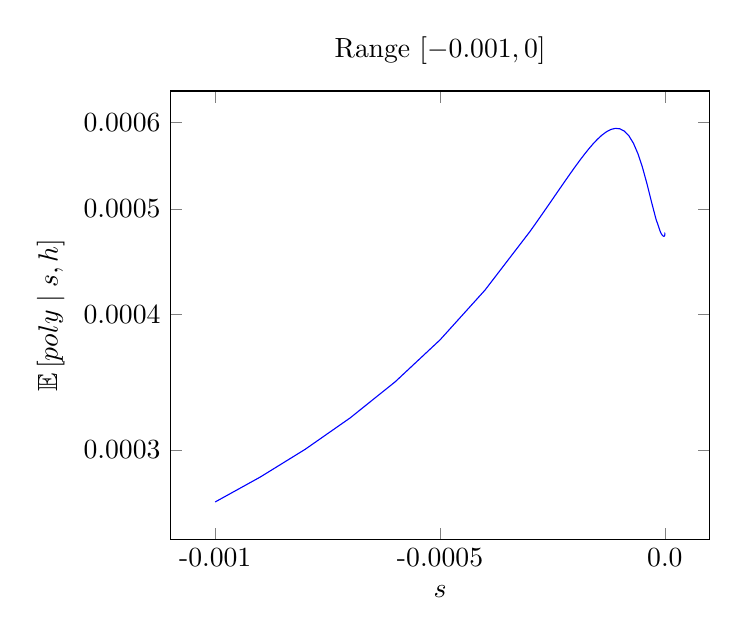
\begin{tikzpicture}
		\begin{semilogyaxis}[
				title = {Range $[-0.001, 0]$},
				ylabel = {$\EE \left[ poly \cond s, h \right]$},
				ytick = {0.0006, 0.0005, 0.0004, 0.0003},
				yticklabels = {0.0006, 0.0005, 0.0004, 0.0003},
				xlabel = {$s$},
				xtick = {-0.001, -0.0005, 0.0},
				xticklabels = {-0.001, -0.0005, 0.0}, scaled x ticks=false,
			]
			\addplot [blue] table {
                                -0.001                  0.00026879175372652444
                                -0.0009                 0.00028331915090015124
                                -0.0008                 0.00030047531130410844
                                -0.0007                 0.0003211379400940495
                                -0.0006                 0.0003466166674521268
                                -0.0005                 0.0003788995834447302
                                -0.0004                 0.0004209537013639709
                                -0.0003                 0.0004765846696792525
                                -0.00029                        0.00048301019846077464
                                -0.00028                        0.0004895903402668485
                                -0.00027                        0.0004963191734383967
                                -0.00026                        0.0005031878886341686
                                -0.00025                        0.0005101840857221512
                                -0.00024                        0.0005172909078969085
                                -0.00023                        0.000524485974114417
                                -0.00022                        0.0005317400623505819
                                -0.00021                        0.0005390154847165423
                                -0.0002                 0.0005462640827368618
                                -0.00019                        0.0005534247574748073
                                -0.00018                        0.0005604204355014928
                                -0.00017                        0.0005671543610822852
                                -0.00016                        0.0005735056087063938
                                -0.00015                        0.0005793237405968988
                                -0.00014                        0.0005844226196004826
                                -0.00013                        0.0005885735941160031
                                -0.00012                        0.0005914986936467291
                                -0.00011                        0.0005928652916217373
                                -0.0001                 0.0005922851736485207
                                -0.00009                        0.0005893235283430916
                                -0.00008                        0.0005835273589598799
                                -0.00007                        0.0005744881951830009
                                -0.00006                        0.000561958801487218
                                -0.00005                        0.0005460416965322386
                                -0.00004                        0.0005274456035118235
                                -0.00003                        0.0005077477505613694
                                -0.00002                        0.0004895112022593879
                                -0.00001                        0.0004760904786845811
                                -0.000009                       0.0004751586534256445
                                -0.000008                       0.0004743189575508033
                                -0.000007                       0.0004735772121025261
                                -0.000006                       0.00047294057062432295
                                -0.000005                       0.00047241857525599193
                                -0.000004                       0.0004720254077002949
                                -0.000003                       0.00047178542815747184
                                -0.000002                       0.0004717502507929271
                                -0.000001                       0.00047207893557613253
                                -0.0000009                      0.0004721505057865423
                                -0.0000008                      0.000472234506840612
                                -0.0000007                      0.0004723339880430206
                                -0.0000006                      0.00047245341081619363
                                -0.0000005                      0.00047259968576005614
                                -0.0000004                      0.00047278438010174735
                                -0.0000003                      0.00047302915859703343
                                -0.0000002                      0.000473382606117568
                                -0.0000001                      0.00047399940914860975
                                -0.00000009                     0.0004740939257882394
                                -0.00000008                     0.00047419971410839277
                                -0.00000007                     0.000474319756924066
                                -0.00000006                     0.0004744584050349582
                                -0.00000005                     0.0004746223431523665
                                -0.00000004                     0.0004748226248735699
                                -0.00000003                     0.0004750325097726186
                                -0.00000002                     0.0004750320834016828
                                -0.00000001                     0.00047503166662056224
                                -0.000000009                    0.00047503162546992835
                                -0.000000008                    0.0004750315844152037
                                -0.000000007                    0.00047503154345638905
                                -0.000000006                    0.0004750315025934855
                                -0.000000005                    0.00047503146182649404
                                -0.000000004                    0.00047503142115541577
                                -0.000000003                    0.0004750313805802515
                                -0.000000002                    0.0004750313401010024
                                -0.000000001                    0.0004750312997176693
                                0                       0.0004750312594302533
			};
		\end{semilogyaxis}
	\end{tikzpicture}
	\caption{Expected polymorphisms in terms of the selection coefficient for $h = 0.0$}
	\label{Figure: Epected poly given s for h = 0.0}
\end{figure}

\begin{figure}[h]
	\centering
	\pgfplotsset{width=5cm}
	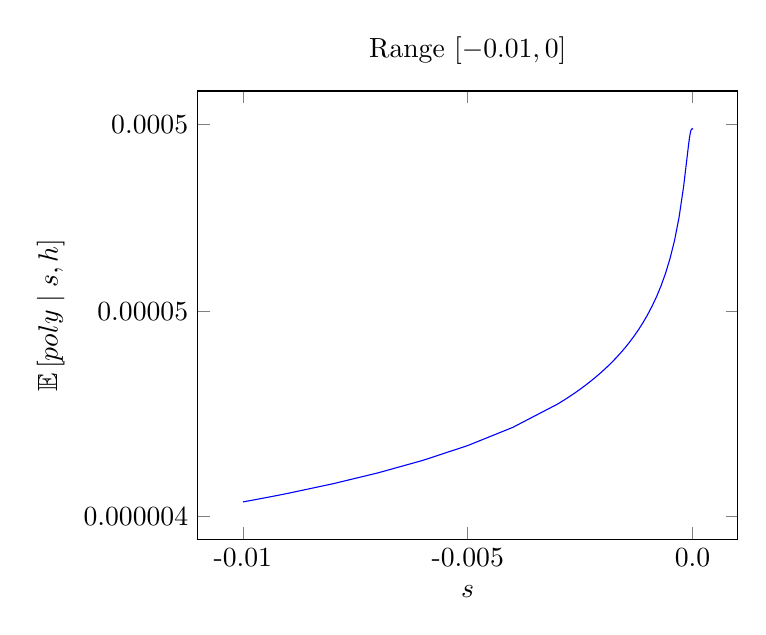
\begin{tikzpicture}
		\begin{semilogyaxis}[
				title = {Range $[-0.01, 0]$},
				ylabel = {$\EE \left[ poly \cond s, h \right]$},
				ytick = {0.0005, 0.00005, 0.000004},
				yticklabels = {0.0005, 0.00005, 0.000004},
				xlabel = {$s$},
				xtick = {-0.01, -0.005, 0.0},
				xticklabels = {-0.01, -0.005, 0.0}, scaled x ticks=false,
			]
			\addplot [blue] table {
                                -0.01                   0.00000479997647734296
                                -0.0099                 0.000004848460849796198
                                -0.0098                 0.000004897934694321415
                                -0.0097                 0.000004948428612993781
                                -0.0096                 0.000004999974482968444
                                -0.0095                 0.000005052605523589654
                                -0.0094                 0.000005106356367783429
                                -0.0093                 0.0000051612631380561735
                                -0.0092                 0.000005217363527449701
                                -0.0091                 0.0000052746968858339345
                                -0.009                  0.000005333304311952395
                                -0.008                  0.000005999963293191994
                                -0.007                  0.000006857094942384255
                                -0.006                  0.000007999934817270792
                                -0.005                  0.0000095999061733932
                                -0.004                  0.000011999853410159282
                                -0.003                  0.000015999739246908358
                                -0.003                  0.000015999739246908358
                                -0.0029                 0.00001655144505689872
                                -0.0028                 0.000017142557728550937
                                -0.0027                 0.000017777455721105884
                                -0.0026                 0.000018461191089860557
                                -0.0025                 0.000019199624202635015
                                -0.0024                 0.00001999959213463359
                                -0.0023                 0.00002086912099141407
                                -0.0022                 0.00002181769613675841
                                -0.0021                 0.000022856609626596203
                                -0.002                  0.00002399941187038822
                                -0.0019                 0.000025262505918491406
                                -0.0018                 0.00002666593983952683
                                -0.0017                 0.000028234478751658876
                                -0.0016                 0.000029999078852260955
                                -0.0015                 0.000031998951038445086
                                -0.0014                 0.000034284508902388816
                                -0.0013                 0.00003692167728299104
                                -0.0012                 0.000039998354993882765
                                -0.0011                 0.00004363440248843787
                                -0.001                  0.000047997621705413985
                                -0.0009                 0.00005333038779169532
                                -0.0008                 0.000059996247514457057
                                -0.0007                 0.00006856640802241289
                                -0.0006                 0.0000799922938937364
                                -0.0005                 0.00009598149826447943
                                -0.0004                 0.00011990395653069087
                                -0.0003                 0.00015918308655767338
                                -0.0002                 0.00023144914603977188
                                -0.0001                 0.0003689547839467094
                                -0.00009                        0.00038626332167114705
                                -0.00008                        0.00040349752196773445
                                -0.00007                        0.0004201601620392659
                                -0.00006                        0.0004356037778139316
                                -0.00005                        0.00044905479445974387
                                -0.00004                        0.0004597081842021377
                                -0.00003                        0.0004669283887963288
                                -0.00002                        0.00047056109317606716
                                -0.00001                        0.0004713150704315243
                                -0.000009                       0.0004712989390215518
                                -0.000008                       0.0004712785733867534
                                -0.000007                       0.00047125907890987106
                                -0.000006                       0.00047124708393578605
                                -0.000005                       0.00047125179956120506
                                -0.000004                       0.0004712872733711276
                                -0.000003                       0.00047137793014515776
                                -0.000002                       0.00047157564794320274
                                -0.000001                       0.00047203994879155167
                                -0.0000009                      0.00047211975383910205
                                -0.0000008                      0.00047221102408015334
                                -0.0000007                      0.00047231680958221005
                                -0.0000006                      0.0004724415725419165
                                -0.0000005                      0.0004725922243355974
                                -0.0000004                      0.00047278033295487803
                                -0.0000003                      0.0004730275638736019
                                -0.0000002                      0.00047338250251230775
                                -0.0000001                      0.00047399983499340576
                                -0.00000009                     0.0004740943515334002
                                -0.00000008                     0.0004742001300432135
                                -0.00000007                     0.0004743201532927273
                                -0.00000006                     0.0004744587720022496
                                -0.00000005                     0.00047462267074529927
                                -0.00000004                     0.0004748229028403376
                                -0.00000003                     0.0004750327284553443
                                -0.00000002                     0.0004750322387486744
                                -0.00000001                     0.0004750317490729935
                                -0.000000009                    0.0004750317001072049
                                -0.000000008                    0.0004750316511417477
                                -0.000000007                    0.0004750316021766237
                                -0.000000006                    0.0004750315532118352
                                -0.000000005                    0.00047503150424738376
                                -0.000000004                    0.0004750314552832716
                                -0.000000003                    0.00047503140631950045
                                -0.000000002                    0.0004750313573560724
                                -0.000000001                    0.00047503130839298937
                                0                       		0.0004750312594302533
			};
		\end{semilogyaxis}
	\end{tikzpicture}
	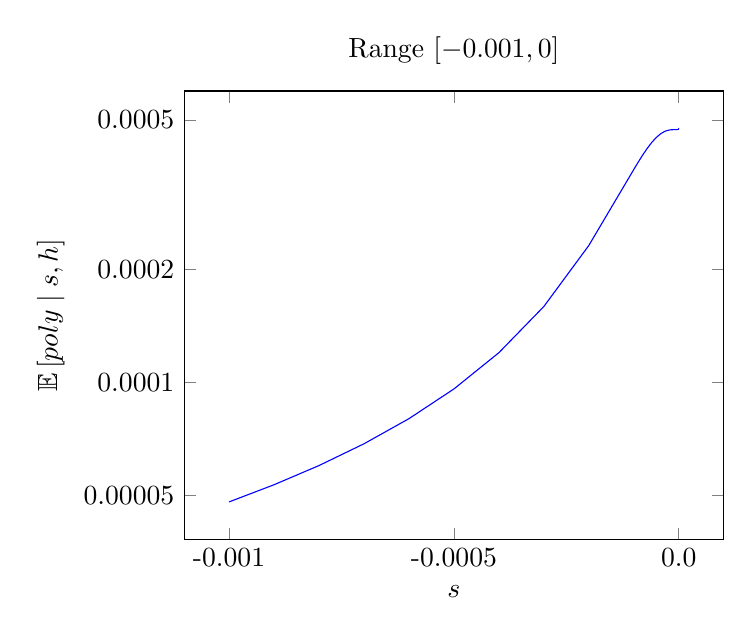
\begin{tikzpicture}
		\begin{semilogyaxis}[
				title = {Range $[-0.001, 0]$},
				ylabel = {$\EE \left[ poly \cond s, h \right]$},
				ytick = {0.0005, 0.0002, 0.0001, 0.00005},
				yticklabels = {0.0005, 0.0002, 0.0001, 0.00005},
				xlabel = {$s$},
				xtick = {-0.001, -0.0005, 0.0},
				xticklabels = {-0.001, -0.0005, 0.0}, 
				scaled x ticks=false,
			]
			\addplot [blue] table {
                                -0.001                  0.000047997621705413985
                                -0.0009                 0.00005333038779169532
                                -0.0008                 0.000059996247514457057
                                -0.0007                 0.00006856640802241289
                                -0.0006                 0.0000799922938937364
                                -0.0005                 0.00009598149826447943
                                -0.0004                 0.00011990395653069087
                                -0.0003                 0.00015918308655767338
                                -0.0002                 0.00023144914603977188
                                -0.0001                 0.0003689547839467094
                                -0.00009                        0.00038626332167114705
                                -0.00008                        0.00040349752196773445
                                -0.00007                        0.0004201601620392659
                                -0.00006                        0.0004356037778139316
                                -0.00005                        0.00044905479445974387
                                -0.00004                        0.0004597081842021377
                                -0.00003                        0.0004669283887963288
                                -0.00002                        0.00047056109317606716
                                -0.00001                        0.0004713150704315243
                                -0.000009                       0.0004712989390215518
                                -0.000008                       0.0004712785733867534
                                -0.000007                       0.00047125907890987106
                                -0.000006                       0.00047124708393578605
                                -0.000005                       0.00047125179956120506
                                -0.000004                       0.0004712872733711276
                                -0.000003                       0.00047137793014515776
                                -0.000002                       0.00047157564794320274
                                -0.000001                       0.00047203994879155167
                                -0.0000009                      0.00047211975383910205
                                -0.0000008                      0.00047221102408015334
                                -0.0000007                      0.00047231680958221005
                                -0.0000006                      0.0004724415725419165
                                -0.0000005                      0.0004725922243355974
                                -0.0000004                      0.00047278033295487803
                                -0.0000003                      0.0004730275638736019
                                -0.0000002                      0.00047338250251230775
                                -0.0000001                      0.00047399983499340576
                                -0.00000009                     0.0004740943515334002
                                -0.00000008                     0.0004742001300432135
                                -0.00000007                     0.0004743201532927273
                                -0.00000006                     0.0004744587720022496
                                -0.00000005                     0.00047462267074529927
                                -0.00000004                     0.0004748229028403376
                                -0.00000003                     0.0004750327284553443
                                -0.00000002                     0.0004750322387486744
                                -0.00000001                     0.0004750317490729935
                                -0.000000009                    0.0004750317001072049
                                -0.000000008                    0.0004750316511417477
                                -0.000000007                    0.0004750316021766237
                                -0.000000006                    0.0004750315532118352
                                -0.000000005                    0.00047503150424738376
                                -0.000000004                    0.0004750314552832716
                                -0.000000003                    0.00047503140631950045
                                -0.000000002                    0.0004750313573560724
                                -0.000000001                    0.00047503130839298937
                                0                       		0.0004750312594302533
			};
		\end{semilogyaxis}
	\end{tikzpicture}
	\caption{Expected polymorphisms in terms of the selection coefficient for $h = 0.5$}
	\label{Figure: Epected poly given s for h = 0.5}
\end{figure}

\paragraph{Random s.}
To compute $\EE[poly]$ where $s$ is random and $h$ is a function of $s$, we simply integrate our approximation of $\EE \left[ poly \cond s, h \right]$ with the corresponding density function of $s$. 
In other words, we compute the following expression
\[
	\EE \left[ poly \right] = \int_{\RR} \EE \left[ poly \cond s, h(s) \right] f_s(s) \, ds \,.
\]

\paragraph{Point mass.}
Consider
\begin{align*}
	s &\equiv s_0 \\
	h &\equiv 0.0
\end{align*}
Then, 
\begin{align*}
	\EE[poly] 
		= \EE \left[ poly \cond S_0, h(S_0) \right]
		\approx 0.000085 \,.
\end{align*}



\paragraph{Gamma distribution.}
Consider 
\begin{align*}
	s &\sim -\Gamma(\alpha, \beta) \\
	h &\equiv 0.5
\end{align*}
Therefore, 
\begin{align*}
	\EE[poly] 
		&= \int_{-\infty}^{0} \EE \left[ poly \cond s, h(s) \right] f_{\Gamma(\alpha, \beta)}(-s) \, ds \,,
\end{align*}
Note that the infinite integral can be approximated by imposing a lower bound since $\Gamma(\alpha, \beta)$ is exponentially decreasing and $\EE \left[ poly \cond s, h(s) \right] \in [0, 1]$, and the bound depends on $\alpha$ and $\beta$.
For example, by Chebyshev's inequality, we have that
\[
	\PP( \Gamma(\alpha, \beta) \ge t ) \le \frac{\alpha}{(t \beta)^2} \,, 
\]
so the lower bound $-0.01$ implies an error of at most $10^{-5}$ as long as $\alpha \le \beta^2 \cdot 10^{-9}$.
By further considering a bound on the value of $\EE [poly | s, h(s)]$, we can deal with more parameters $\alpha, \beta$.

Lastly, while the density $f_{\Gamma(\alpha, \beta)}(\cot)$ is generally difficult to evaluate, the cummulative density $F_{\Gamma(\alpha, \beta)}(\cot)$ is easier to evaluate numerically.
Therefore, we consider the following approximation
\[
	\EE[poly] 
			\approx \sum_{i = 1}^{n - 1} \big( F_{\Gamma(\alpha, \beta)}(s_{i + 1}) - F_{\Gamma(\alpha, \beta)}(s_{i}) \big) \EE \left[ poly \cond -s_{i}, h(-s_{i}) \right] \,,
\]
where $0 = s_0 < s_1 < \ldots < s_n$ is an appropiate grid.
This approximation correspond to approximate $s \mapsto \EE \left[ poly \cond s, h(s) \right]$ by a function that is constant by parts.
Considering previous approximations, we can choose a grid so that the overall error is less than $10^{-5}$.
See \Cref{Figure: Approximation alpah = 1} for an illustration.

\begin{figure}[h]
	\centering
	\pgfplotsset{width=7cm}
	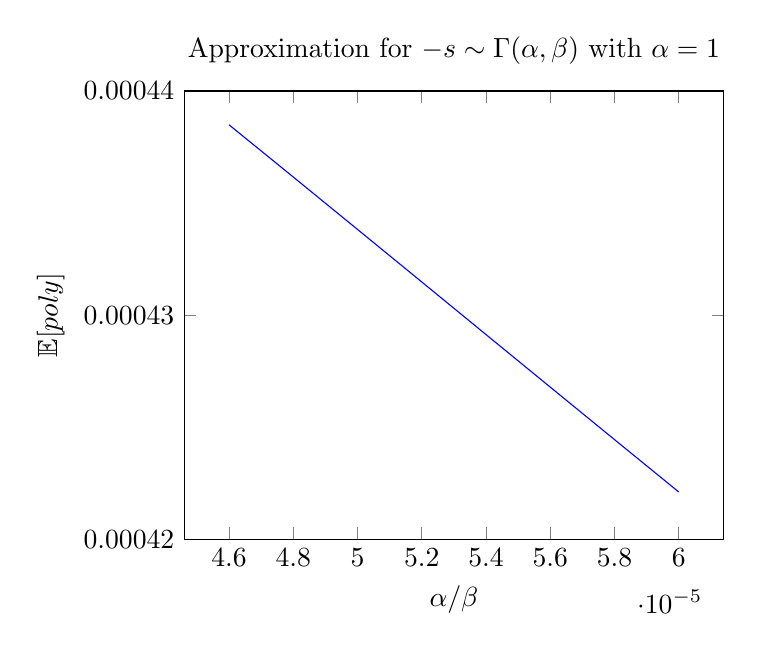
\begin{tikzpicture}
		\begin{axis}[
				title = {Approximation for $-s \sim \Gamma(\alpha, \beta)$ with  $\alpha = 1$},
				xlabel = {$\alpha/\beta$},
	%			xtick = {0.0001, 0.00000001, 0.000000000001, 0.0000000000000001},
				ylabel = {$\EE[poly]$},
				ymax = {0.00044},
				ymin = {0.00042},
				ytick = {0.00044, 0.00043, 0.00042},
				yticklabels = {0.00044, 0.00043, 0.00042},
				scaled y ticks=false,
			]
			\addplot [blue] table {
				0.000046 0.0004384899
				0.000048 0.0004361606
				0.00005 0.0004338224
				0.000052 0.0004314789
				0.000054 0.0004291332
				0.000056 0.0004267884
				0.000058 0.0004244470
				0.00006 0.0004221110
			};
		\end{axis}
	\end{tikzpicture}
	\caption{Expected polymorphisms for gamma distributed selection coefficient}
	\label{Figure: Approximation alpah = 1}
\end{figure}


\section{Examples}

In this section we compute $\EE[poly]$ explictly for one parameter choice. 
Consider the case $p = 0.5$, $\alpha = 10$, and $\beta = 2 \cdot 10^4$.
Note that
\[
	\EE[ poly ] = p \EE[ poly | s = S_0, h = 0] + (1 - p) \EE_{-s \sim \Gamma(\alpha, \beta)} [ \EE[ poly | s, h = 0.5] ] \,.
\]
Since
\begin{align*}
	\EE[ poly | s = S_0, h = 0] 
		&\approx 0.0000850151 \\
	\EE_{-s \sim \Gamma(\alpha, \beta)} [ \EE[ poly | s, h = 0.5] ]
		&\approx 0.0001073323
\end{align*}
we get that
\[
	\EE[ poly ] \approx 0.0000961737 \,.
\]







\section{Numerical evaluations}

Our parametric model depends on $p$, $\alpha$ and $\beta$.
We explore the space of all possible values by computing the expected polymorphisms only on a selected choice of parameters.

% Table generator
% https://tableconvert.com/csv-to-latex


\begin{longtable}{|l|l|l|c|}
   	\hline
   	$p$ & $\alpha$ & $1 / \beta$ & expected polymorphisms \\ \hline \hline
		0 & 300.0000000000001 & 0.0000001541467657920456 & 0.0004530 \\ \hline
        0 & 300.0000000000001 & 0.0000001541467657920456 & 0.0004530 \\ \hline
        0 & 290.8506518295917 & 0.0000001584893192461114 & 0.0004532 \\ \hline
        0 & 225.56161320737237 & 0.0000002059863942616875 & 0.0004528 \\ \hline
        0 & 182.5276007813775 & 0.00000025118864315095823 & 0.0004534 \\ \hline
        0 & 169.59347117570735 & 0.0000002708036442160055 & 0.0004533 \\ \hline
        0 & 127.51258982610176 & 0.0000003652004813843986 & 0.0004525 \\ \hline
        0 & 115.93811031632079 & 0.00000039810717055349687 & 0.0004530 \\ \hline
        0 & 95.87315155141827 & 0.0000004836048047249234 & 0.0004527 \\ \hline
        0 & 72.81762821148743 & 0.000000630957344480193 & 0.0004530 \\ \hline
        0 & 72.08434242404265 & 0.0000006376784776269807 & 0.0004530 \\ \hline
        0 & 54.19820188053225 & 0.000000862049856020774 & 0.0004520 \\ \hline
        0 & 46.27986268057486 & 0.0000009999999999999997 & 0.0004524 \\ \hline
        0 & 40.750112830372316 & 0.0000011416356918193267 & 0.0004521 \\ \hline
        0 & 30.638870628004046 & 0.0000015174645544368143 & 0.0004518 \\ \hline
        0 & 29.267338838171042 & 0.000001584893192461114 & 0.0004519 \\ \hline
        0 & 23.036510285681892 & 0.0000020426117609592174 & 0.0004509 \\ \hline
        0 & 18.58524958360993 & 0.0000025118864315095823 & 0.0004510 \\ \hline
        0 & 17.320508075688775 & 0.0000027076390188324098 & 0.0004506 \\ \hline
        0 & 13.022805810412262 & 0.0000036300647024173715 & 0.0004497 \\ \hline
        0 & 11.84596516073017 & 0.000003981071705534969 & 0.0004496 \\ \hline
        0 & 9.791483623609768 & 0.000004887475719264104 & 0.0004483 \\ \hline
        0 & 7.549938308749734 & 0.00000630957344480193 & 0.0004477 \\ \hline
        0 & 7.3619428061166206 & 0.000006487995060251171 & 0.0004475 \\ \hline
        0 & 5.535238985626912 & 0.00000880608239687674 & 0.0004453 \\ \hline
        0 & 4.874872287742436 & 0.00001 & 0.0004447 \\ \hline
        0 & 4.161791450287818 & 0.000011941732589246017 & 0.0004429 \\ \hline
        0 & 3.151143795792919 & 0.000015848931924611138 & 0.0004411 \\ \hline
        0 & 3.1291346445318977 & 0.000015980727030317896 & 0.0004410 \\ \hline
        0 & 2.3527088612123075 & 0.000022084851528262447 & 0.0004370 \\ \hline
        0 & 2.0796912080337586 & 0.000025118864315095822 & 0.0004359 \\ \hline
        0 & 1.7689360204744258 & 0.000030532846214531185 & 0.0004326 \\ \hline
        0 & 1.386785662694208 & 0.000039810717055349695 & 0.0004296 \\ \hline
        0 & 1.3300135414628025 & 0.000042040057592132016 & 0.0004285 \\ \hline
        0 & 1 & 0.000059268778545316244 & 0.0004230 \\ \hline
        0.1 & 300.0000000000001 & 0.00000012221738250849407 & 0.0004244 \\ \hline
        0.1 & 300.0000000000001 & 0.00000012221738250849407 & 0.0004244 \\ \hline
        0.1 & 225.56161320737237 & 0.00000015745614479235895 & 0.0004251 \\ \hline
        0.1 & 224.1010946598654 & 0.0000001584893192461114 & 0.0004251 \\ \hline
        0.1 & 169.59347117570732 & 0.0000002144465552856113 & 0.0004245 \\ \hline
        0.1 & 143.34770274920493 & 0.00000025118864315095823 & 0.0004248 \\ \hline
        0.1 & 127.51258982610176 & 0.00000028579681663925166 & 0.0004245 \\ \hline
        0.1 & 95.87315155141827 & 0.00000037423151438881107 & 0.0004248 \\ \hline
        0.1 & 90.0283006949983 & 0.0000003981071705534969 & 0.0004248 \\ \hline
        0.1 & 72.08434242404266 & 0.0000005083976144022012 & 0.0004242 \\ \hline
        0.1 & 57.05958587182932 & 0.000000630957344480193 & 0.0004246 \\ \hline
        0.1 & 54.19820188053225 & 0.0000006666962666444516 & 0.0004245 \\ \hline
        0.1 & 40.750112830372316 & 0.0000008930699466512873 & 0.0004242 \\ \hline
        0.1 & 36.22876263209082 & 0.000001 & 0.0004242 \\ \hline
        0.1 & 30.63887062800405 & 0.0000011993468186386521 & 0.0004237 \\ \hline
        0.1 & 23.036510285681896 & 0.0000015714416165845784 & 0.0004239 \\ \hline
        0.1 & 22.837445924637542 & 0.000001584893192461114 & 0.0004239 \\ \hline
        0.1 & 17.320508075688775 & 0.0000021300562536844447 & 0.0004231 \\ \hline
        0.1 & 14.603973433793314 & 0.0000025118864315095823 & 0.0004231 \\ \hline
        0.1 & 13.02280581041226 & 0.0000028419398537103077 & 0.0004227 \\ \hline
        0.1 & 9.791483623609768 & 0.0000037781975987967553 & 0.0004222 \\ \hline
        0.1 & 9.284429639760333 & 0.000003981071705534969 & 0.0004221 \\ \hline
        0.1 & 7.36194280611662 & 0.000005109136821319283 & 0.0004211 \\ \hline
        0.1 & 5.947353627019855 & 0.00000630957344480193 & 0.0004206 \\ \hline
        0.1 & 5.535238985626913 & 0.000006827122654861981 & 0.0004201 \\ \hline
        0.1 & 4.161791450287818 & 0.00000918627914562949 & 0.0004187 \\ \hline
        0.1 & 3.8238639591838774 & 0.00001 & 0.0004184 \\ \hline
        0.1 & 3.129134644531898 & 0.000012482821607816822 & 0.0004168 \\ \hline
        0.1 & 2.475753088277439 & 0.00001584893192461114 & 0.0004155 \\ \hline
        0.1 & 2.3527088612123075 & 0.000016813321581146697 & 0.0004149 \\ \hline
        0.1 & 1.7689360204744258 & 0.00002294015464650834 & 0.0004123 \\ \hline
        0.1 & 1.6201389072592205 & 0.000025118864315095822 & 0.0004116 \\ \hline
        0.1 & 1.3300135414628023 & 0.00003168060528558289 & 0.0004090 \\ \hline
        0.1 & 1.0756784679359217 & 0.000039810717055349695 & 0.0004069 \\ \hline
        0.1 & 1 & 0.000043676489470296766 & 0.0004056 \\ \hline
        0.2 & 256.2807710325777 & 0.0000001 & 0.0003918 \\ \hline
        0.2 & 256.2807710325777 & 0.0000001 & 0.0003918 \\ \hline
        0.2 & 225.56161320737237 & 0.00000011364696122304818 & 0.0003918 \\ \hline
        0.2 & 169.59347117570735 & 0.00000015123953747595992 & 0.0003918 \\ \hline
        0.2 & 161.96443250931463 & 0.0000001584893192461114 & 0.0003918 \\ \hline
        0.2 & 127.51258982610179 & 0.00000020055942186273017 & 0.0003918 \\ \hline
        0.2 & 102.14031138870588 & 0.00000025118864315095823 & 0.0003918 \\ \hline
        0.2 & 95.87315155141827 & 0.00000026824058482269253 & 0.0003918 \\ \hline
        0.2 & 72.08434242404265 & 0.00000035497809161196566 & 0.0003918 \\ \hline
        0.2 & 64.36502993948046 & 0.0000003981071705534969 & 0.0003918 \\ \hline
        0.2 & 54.19820188053225 & 0.00000047318691333941774 & 0.0003917 \\ \hline
        0.2 & 40.750112830372316 & 0.0000006294673535524286 & 0.0003917 \\ \hline
        0.2 & 40.65347306971581 & 0.000000630957344480193 & 0.0003917 \\ \hline
        0.2 & 30.63887062800405 & 0.0000008365144655244301 & 0.0003916 \\ \hline
        0.2 & 25.639846151723688 & 0.000001 & 0.0003916 \\ \hline
        0.2 & 23.036510285681896 & 0.0000011178082096049572 & 0.0003915 \\ \hline
        0.2 & 17.320508075688775 & 0.0000014822120906896504 & 0.0003914 \\ \hline
        0.2 & 16.194502664483952 & 0.000001584893192461114 & 0.0003914 \\ \hline
        0.2 & 13.022805810412258 & 0.0000019836209570038384 & 0.0003912 \\ \hline
        0.2 & 10.253734393489943 & 0.0000025118864315095823 & 0.0003910 \\ \hline
        0.2 & 9.791483623609768 & 0.0000026384100777932896 & 0.0003909 \\ \hline
        0.2 & 7.3619428061166206 & 0.00000352472795994203 & 0.0003906 \\ \hline
        0.2 & 6.510512597897407 & 0.000003981071705534969 & 0.0003905 \\ \hline
        0.2 & 5.535238985626911 & 0.000004726606709275465 & 0.0003901 \\ \hline
        0.2 & 4.161791450287818 & 0.0000062733360853971586 & 0.0003897 \\ \hline
        0.2 & 4.137573074316612 & 0.00000630957344480193 & 0.0003896 \\ \hline
        0.2 & 3.129134644531898 & 0.00000845758051600518 & 0.0003888 \\ \hline
        0.2 & 2.643460952791566 & 0.00001 & 0.0003884 \\ \hline
        0.2 & 2.3527088612123075 & 0.000011347301376863671 & 0.0003879 \\ \hline
        0.2 & 1.7689360204744258 & 0.000015164806245905173 & 0.0003868 \\ \hline
        0.2 & 1.6917548381801009 & 0.00001584893192461114 & 0.0003867 \\ \hline
        0.2 & 1.3300135414628025 & 0.00002056177337299613 & 0.0003853 \\ \hline
        0.2 & 1.0917428030640703 & 0.00002511886431509582 & 0.0003844 \\ \hline
        0.2 & 1 & 0.000027786981581076333 & 0.0003837 \\ \hline
        0.3 & 131.73101632587696 & 0.0000001 & 0.0003553 \\ \hline
        0.3 & 131.73101632587696 & 0.0000001 & 0.0003553 \\ \hline
        0.3 & 127.51258982610177 & 0.0000001036031327225367 & 0.0003552 \\ \hline
        0.3 & 95.87315155141827 & 0.00000013560818222650752 & 0.0003553 \\ \hline
        0.3 & 82.91681924936498 & 0.0000001584893192461114 & 0.0003553 \\ \hline
        0.3 & 72.08434242404265 & 0.00000018379256714765547 & 0.0003552 \\ \hline
        0.3 & 54.19820188053225 & 0.00000024049898594786135 & 0.0003553 \\ \hline
        0.3 & 52.162340819646396 & 0.00000025118864315095823 & 0.0003553 \\ \hline
        0.3 & 40.750112830372316 & 0.0000003206455565491242 & 0.0003553 \\ \hline
        0.3 & 32.987505571800696 & 0.0000003981071705534969 & 0.0003552 \\ \hline
        0.3 & 30.638870628004042 & 0.00000043005407274758674 & 0.0003552 \\ \hline
        0.3 & 23.036510285681896 & 0.0000005621415666214232 & 0.0003553 \\ \hline
        0.3 & 20.647798282350223 & 0.000000630957344480193 & 0.0003552 \\ \hline
        0.3 & 17.320508075688775 & 0.000000751704200002037 & 0.0003552 \\ \hline
        0.3 & 13.023131078147005 & 0.000001 & 0.0003552 \\ \hline
        0.3 & 13.02280581041226 & 0.0000010000253540123269 & 0.0003552 \\ \hline
        0.3 & 9.791483623609768 & 0.0000013084998663927643 & 0.0003552 \\ \hline
        0.3 & 8.090646325469281 & 0.000001584893192461114 & 0.0003552 \\ \hline
        0.3 & 7.3619428061166206 & 0.0000017381939942229566 & 0.0003552 \\ \hline
        0.3 & 5.535238985626912 & 0.00000227819286184552 & 0.0003551 \\ \hline
        0.3 & 5.01313317811982 & 0.0000025118864315095823 & 0.0003551 \\ \hline
        0.3 & 4.161791450287818 & 0.000002992023861936028 & 0.0003551 \\ \hline
        0.3 & 3.129134644531898 & 0.000003941117170750688 & 0.0003550 \\ \hline
        0.3 & 3.0963385271032418 & 0.000003981071705534969 & 0.0003550 \\ \hline
        0.3 & 2.3527088612123075 & 0.0000051142938718884704 & 0.0003550 \\ \hline
        0.3 & 1.883291180781875 & 0.00000630957344480193 & 0.0003549 \\ \hline
        0.3 & 1.7689360204744258 & 0.000006694418211172288 & 0.0003549 \\ \hline
        0.3 & 1.3300135414628025 & 0.000008679788297386442 & 0.0003547 \\ \hline
        0.3 & 1.1403134896010028 & 0.000009999999999999999 & 0.0003547 \\ \hline
        0.3 & 1 & 0.000011305223895756521 & 0.0003546 \\ \hline
\end{longtable}

\bibliographystyle{alpha}
\bibliography{refs}


\end{document}